
\begin{figure}
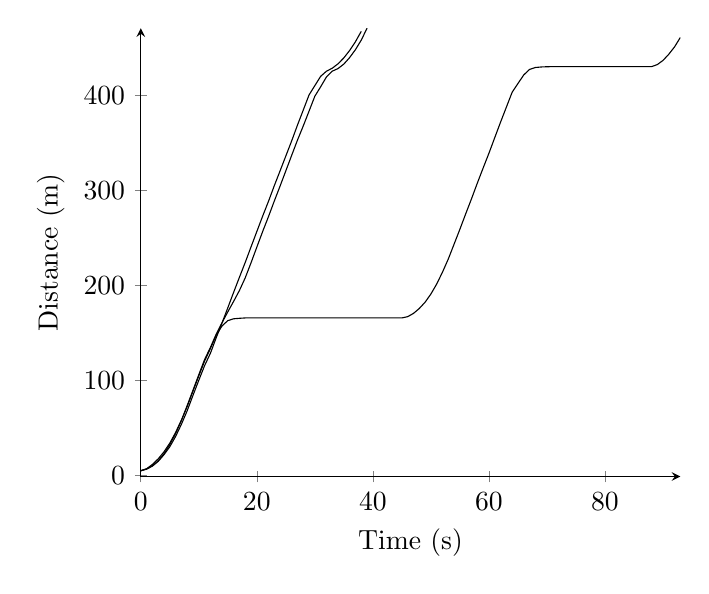
\begin{tikzpicture}
\begin{axis}[
legend style={anchor=west},
axis x line=bottom,
axis y line=left,
ymin=-1,
xlabel=Time (s),
ylabel=Distance (m),
]
\addplot[] coordinates {
(0, 5.1)
(1, 6.94239168768)
(2, 10.2887373731)
(3, 15.5004475966)
(4, 22.8817805266)
(5, 32.5001598192)
(6, 44.2188966157)
(7, 57.7230636434)
(8, 73.6376506916)
(9, 89.7201969127)
(10, 106.038193656)
(11, 121.990325351)
(12, 134.708298756)
(13, 148.688691565)
(14, 160.692825102)
(15, 172.132960314)
(16, 183.157216047)
(17, 194.572098513)
(18, 207.873463015)
(19, 223.658216351)
(20, 240.169699599)
(21, 256.52715263)
(22, 272.126575956)
(23, 288.463325565)
(24, 304.253458063)
(25, 320.413678367)
(26, 336.582007843)
(27, 352.617225294)
(28, 367.5316527)
(29, 383.159860256)
(30, 398.863991693)
(31, 408.759809195)
(32, 419.114869781)
(33, 425.186000594)
(34, 427.959748478)
(35, 432.683824964)
(36, 439.519023579)
(37, 447.843757483)
(38, 457.868804664)
(39, 470.355469269)
};
\addplot[] coordinates {
(0, 5.1)
(1, 7.1682630103)
(2, 11.7233335913)
(3, 17.5705366939)
(4, 24.951678104)
(5, 34.0774190611)
(6, 45.2566759226)
(7, 58.3174272809)
(8, 72.631879333)
(9, 88.8394433948)
(10, 104.823975443)
(11, 120.388056065)
(12, 133.580909142)
(13, 147.549865243)
(14, 157.323967612)
(15, 162.922411579)
(16, 164.848221436)
(17, 165.365438336)
(18, 165.746627806)
(19, 165.757206722)
(20, 165.757206722)
(21, 165.757206722)
(22, 165.757206722)
(23, 165.757206722)
(24, 165.757206722)
(25, 165.757206722)
(26, 165.757206722)
(27, 165.757206722)
(28, 165.757206722)
(29, 165.757206722)
(30, 165.757206722)
(31, 165.757206722)
(32, 165.757206722)
(33, 165.757206722)
(34, 165.757206722)
(35, 165.757206722)
(36, 165.757206722)
(37, 165.757206722)
(38, 165.757206722)
(39, 165.757206722)
(40, 165.757206722)
(41, 165.757206722)
(42, 165.757206722)
(43, 165.757206722)
(44, 165.757206722)
(45, 165.757206722)
(46, 167.11137931)
(47, 170.52948031)
(48, 175.682454858)
(49, 182.307422606)
(50, 190.884853974)
(51, 201.394362465)
(52, 213.905283147)
(53, 227.71793584)
(54, 243.373337566)
(55, 259.035979191)
(56, 275.224591125)
(57, 291.025364089)
(58, 307.45939613)
(59, 323.295205366)
(60, 338.86390079)
(61, 355.236468362)
(62, 371.506313156)
(63, 387.253441255)
(64, 402.987281272)
(65, 412.187541235)
(66, 421.217072499)
(67, 427.004972396)
(68, 429.036558438)
(69, 429.607947119)
(70, 429.877365129)
(71, 429.93620986)
(72, 429.946990023)
(73, 429.946990023)
(74, 429.946990023)
(75, 429.946990023)
(76, 429.946990023)
(77, 429.946990023)
(78, 429.946990023)
(79, 429.946990023)
(80, 429.946990023)
(81, 429.946990023)
(82, 429.946990023)
(83, 429.946990023)
(84, 429.946990023)
(85, 429.946990023)
(86, 429.946990023)
(87, 429.946990023)
(88, 429.946990023)
(89, 432.035712885)
(90, 436.503962922)
(91, 443.012331699)
(92, 450.799573701)
(93, 460.762290414)
};
\addplot[] coordinates {
(0, 5.1)
(1, 6.7532252531)
(2, 9.94820267709)
(3, 14.953140107)
(4, 21.948145512)
(5, 30.2901471755)
(6, 41.1023231604)
(7, 53.8652706786)
(8, 68.1937558916)
(9, 84.3531172742)
(10, 100.182388283)
(11, 115.633057215)
(12, 128.554525331)
(13, 144.915525206)
(14, 160.43277294)
(15, 176.410719517)
(16, 192.620442672)
(17, 208.482798153)
(18, 224.074983558)
(19, 240.410221693)
(20, 256.569146767)
(21, 272.700920827)
(22, 288.180077458)
(23, 304.589923924)
(24, 320.243501553)
(25, 336.005491748)
(26, 351.806804674)
(27, 368.382608684)
(28, 384.240668454)
(29, 400.205651404)
(30, 410.008189166)
(31, 419.778111077)
(32, 425.181883718)
(33, 428.305584488)
(34, 432.943964627)
(35, 439.192575036)
(36, 446.982110576)
(37, 456.183797089)
(38, 467.083340933)
};

\end{axis}
\end{tikzpicture}
\label{tik:0:98}
\caption{0 percent diving with GSC on route $98$}
\end{figure}
